\section{Mission}

\paragraph{Description}
L'entreprise ProBespoke détenais des solutions technologiques mises en place en 2014.
Cependant une absence de suivi et de maintenance et fortement dégradé le système. L'entreprise possède deux sites vitrines, www.bgc.paris et www. probespoke.com, qui sont statiques et demande donc peu d'entretien.
Probespoke a également mis en place une application disponible sur IOs et Android relié à une plateforme ERP (entreprise resource planing). Cette plateforme est construite avec le logiciel open-source odoo.
 Toutes ces solutions sont sur des serveurs AWS (Amazon Web Service) dont les tarifs obscurs ont mal été compris.
\subsection{Travaux technique}
\paragraph{}
 Ma première mission fut de migrer ces serveurs d'AWS vers les serveurs de l'entreprise OVH et faire ainsi passer les coûts fixes d'informatique de l'entreprise de \$1800 à \$500.
 Pendant cette migration j'ai dû également mettre la dernière version de Odoo, pour passer de Odoo 8 à Odoo 11.
 Lors de cette mise à jour des modules codés il y a quatre ans se sont mis à dysfonctionner, j'ai donc dû en recoder une bonne partie. Finalement j'ai rajouté une fonctionnalité de prise de commande rapide sur l'application et permis sa rediffusion.
 \paragraph{}

 \begin{figure}[!h]
 \centering
 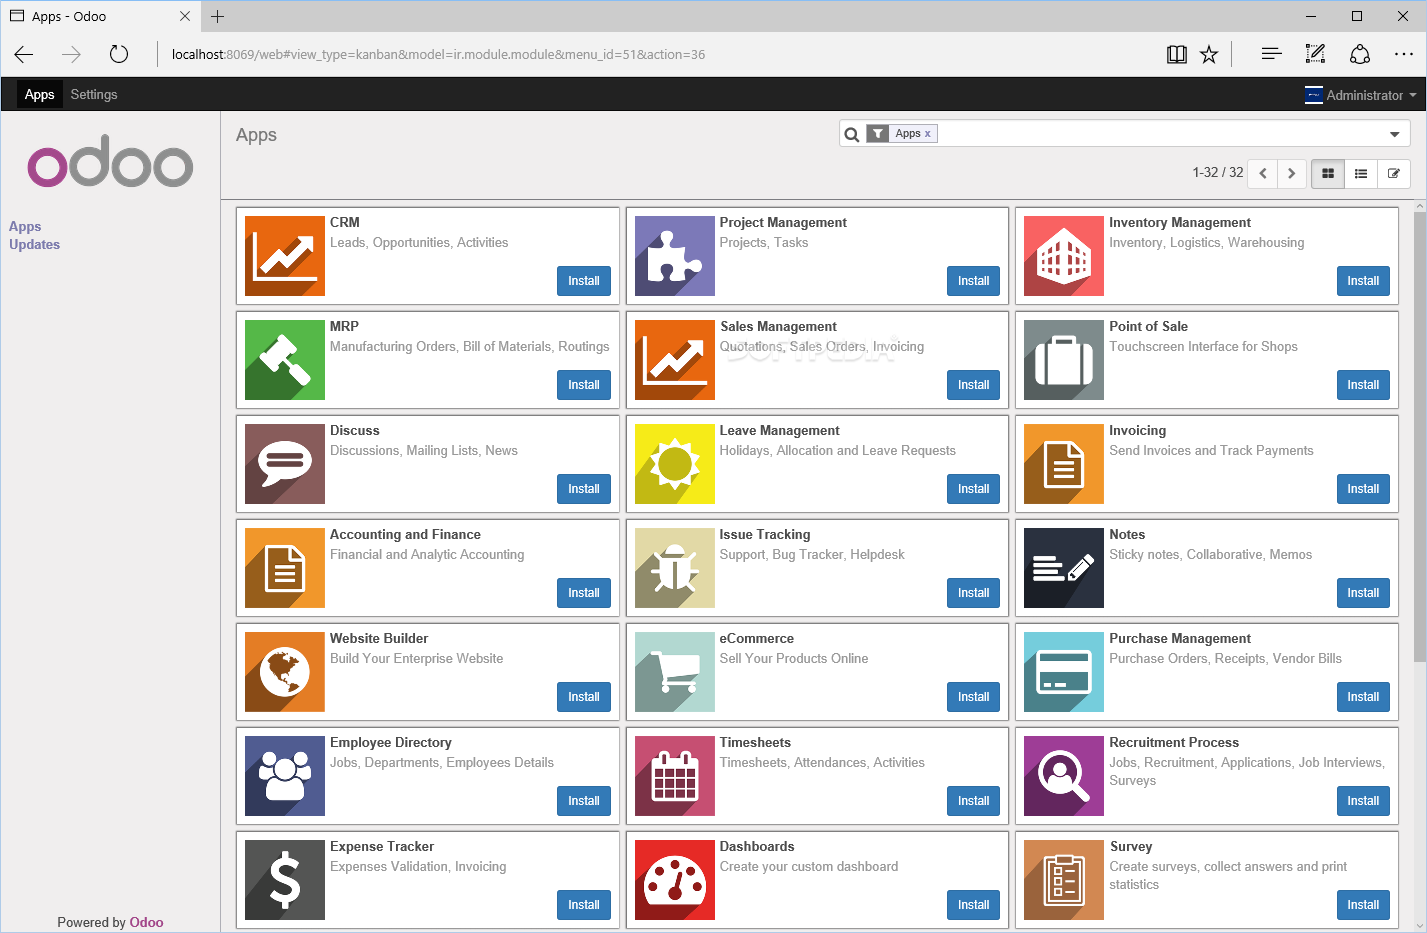
\includegraphics[width=12cm]{image/odoo.png}
 \caption{Différents modules proposés par Odoo}
 \end{figure}

 \subsection{Conseil à l'entreprise}
 \paragraph{}
 Notre employeur n'a pas pour spécialité l'informatique. Ainsi j'ai dû faire des benchmarck pour trouver par exemple la solution d'hébergement de ses serveurs qui sera la moins chers. Je l'ai également mis en garde à propos de certain avancés technologiques qui le pousseront à moyen terme à une réorganisation de ses services. Finalement il m'a également été sollicité pour aider à écrire une demande de devis pour poursuivre la mise en place de son système informatique. Etant pris par son rôle commercial, notre employeur n'a peu de temps pour s'intéresse aux avancés technologiques. De plus ProBespoke n'engage pas d'informaticien à temps plein, ainsi les avancés dans ce domaine sont saccadées. De mon point de vue cela est une erreur étant donné la place prédominante de l'informatique dans cette entreprise.
 \paragraph{}
 \begin{figure}[!h]
 \centering
 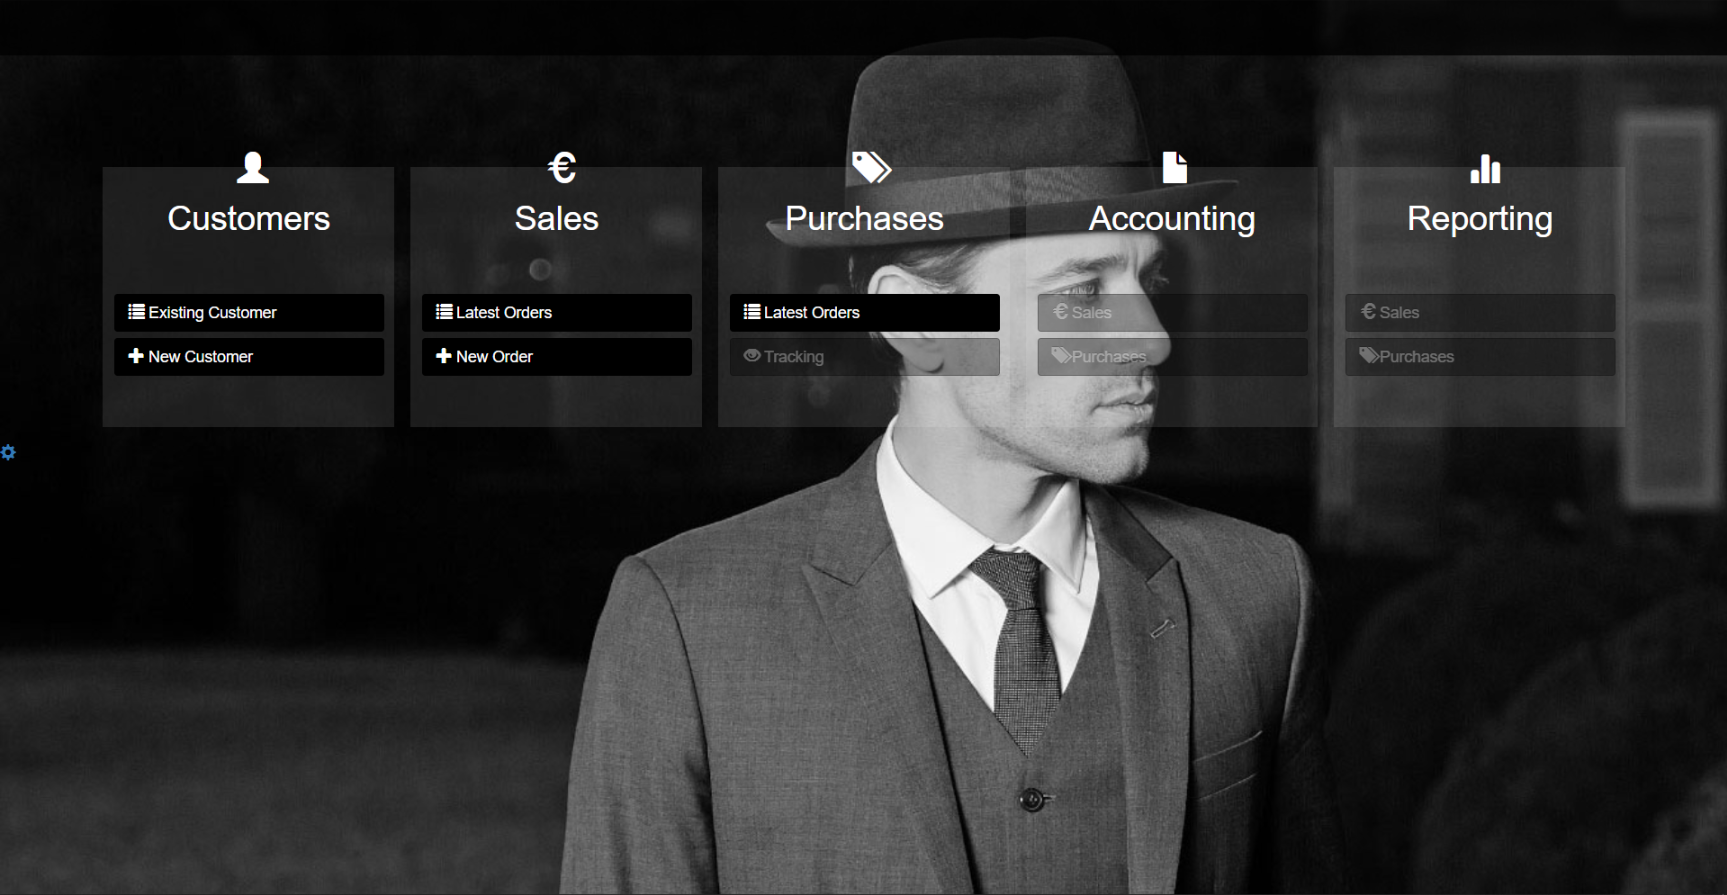
\includegraphics[width=16cm]{image/prise.png}
 \caption{Application de prise de commande}
 \end{figure}

  \subsection{Cadre de travail}
  \paragraph{}
L'entreprise ProBespoke a eu, au cours de son existence, plusieurs prestataires chargés de développer la partie informatique. Ainsi au début une personne nommé Guillaume (je n'ai jamais eu son nom de famille) développa l'application et le logiciel de gestion. Cependant pour une raison que je devine mal un désaccord c'est installé entre lui et M. Saksa le créateur. Puis ProBespoke est passé par une agence pour remettre en place le site internet qui avait besoin de maintenance. Cependant les tarifs étaient prohibitifs pour une petite entreprise comme ProBespoke.
  \paragraph{}
  C'est pourquoi il fut choisi de prendre deux stagiaires ayant des compétences en informatique, ce qui tombait bien car M. Saksa avait pour habitude de vendre des costumes dans des écoles d'ingénieurs. Comment persuader des stagiaires de venir travailler dans son entreprise. Il fut décidé qu'aucun salaire ne serait versé, en revanche le cadre de travail devait être idéal. Ainsi nous eûmes droit à un appartement avec piscine, gym et sauna, quelques repas au restaurant et parfois des soirées au golf. D'un autre côté les horaires était très variables et les journées pouvait être longue et il fallait rester en alerte même le week-end. Cela m'a fait prendre conscience que le salaire est loin d'être la seule variable dans le choix d'un emploie. \begin{figure}[!h]
   \centering
   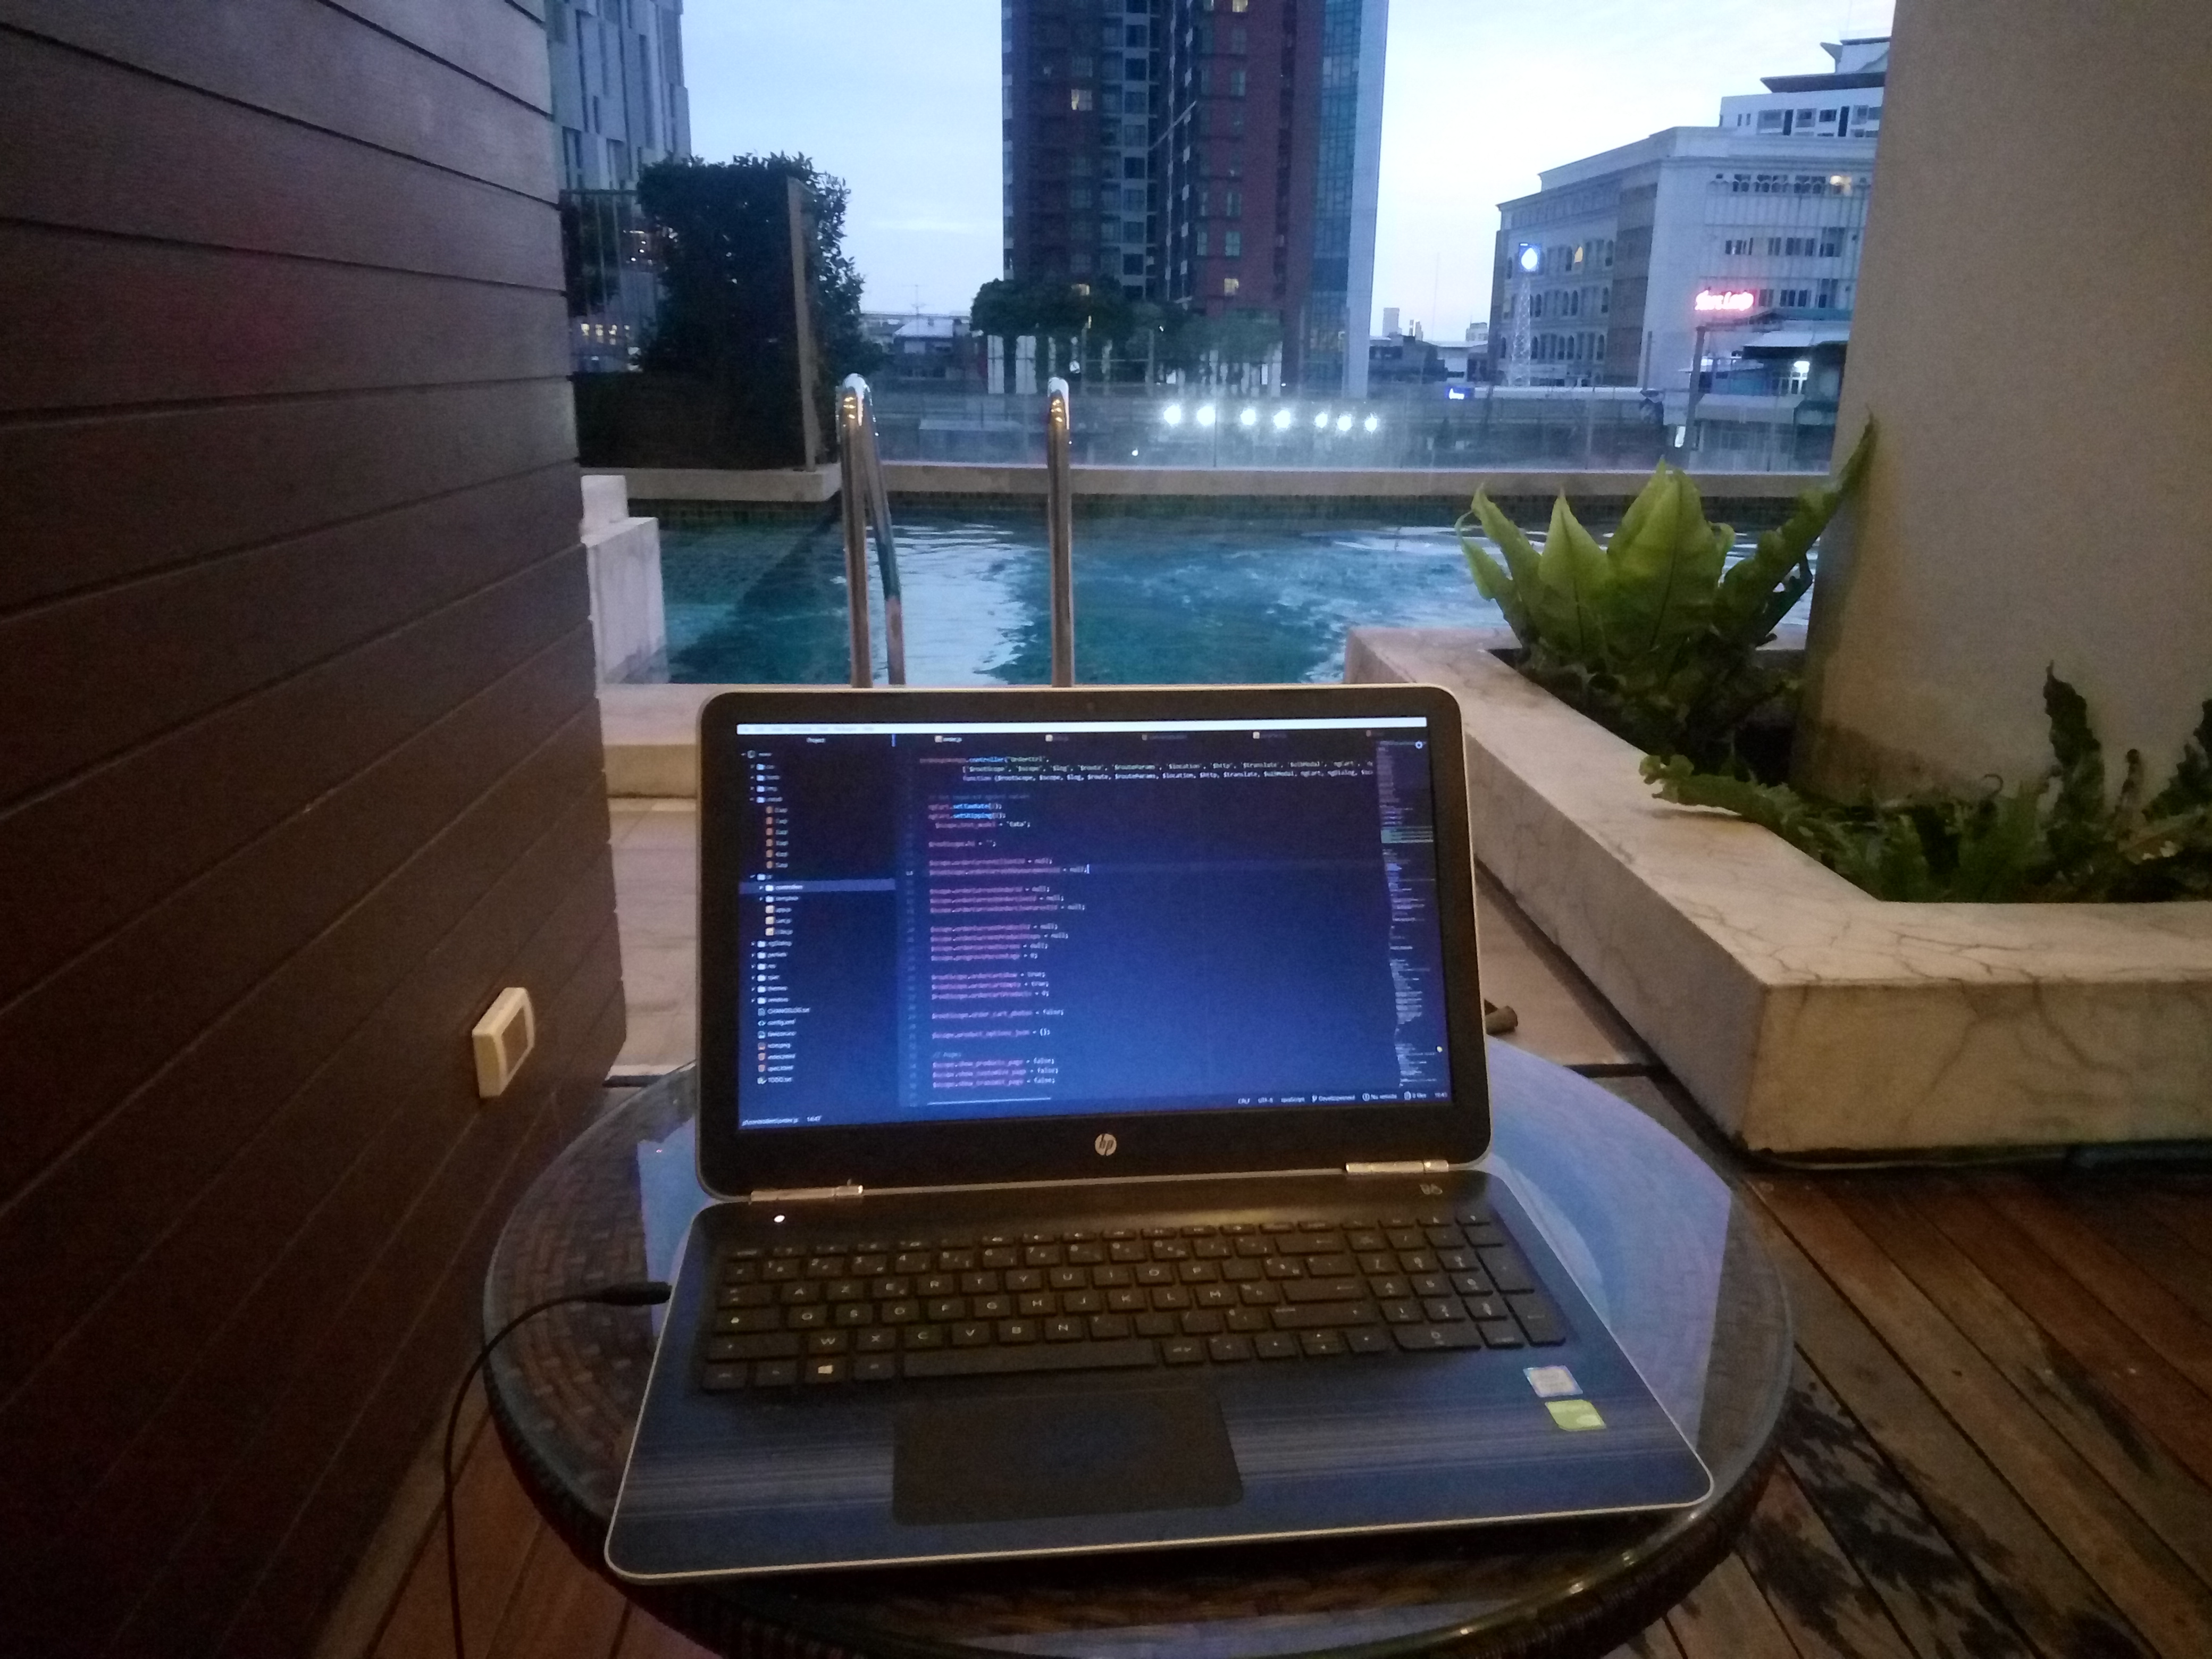
\includegraphics[width=12cm]{image/piscine.jpg}
   \caption{Programmation au bord de la piscine}
   \end{figure}
\paragraph{}
J'aimerais également revenir sur la dispute entre M.Saksa et son précèdent informaticien Guillaume. En effet à cause de cet évènement, ils nous étaient difficile d'avoir un historique de ce qui avait été fait car la personne la mieux placée pour témoigner n'était plus là. Le code était peu documenté, et les explications parfois obscures et incomplète. Nous avons dû une fois écrire un mail au fameux Guillaume ce qui mit fortement mal à l'aise notre patron qui ne voulait pas s'abaisser à lui demander quelque chose. J'en retire également un enseignement. Toujours demander à ses employés de laisser une trace explicative de leurs travaux et toujours essayer de se quitter en bon terme surtout quand cela touche une partie critique de l'entreprise.
